\section{Failure analysis }
\label{sec:why_llms_bad}
In this section, we analyze {\em how} existing  state-of-the-art LLM-assisted systems fail at multi-host red team exercises. These insights help  inform our design of \sys.

\subsection{Methodology}
\begin{figure}[tb]
    \centering
    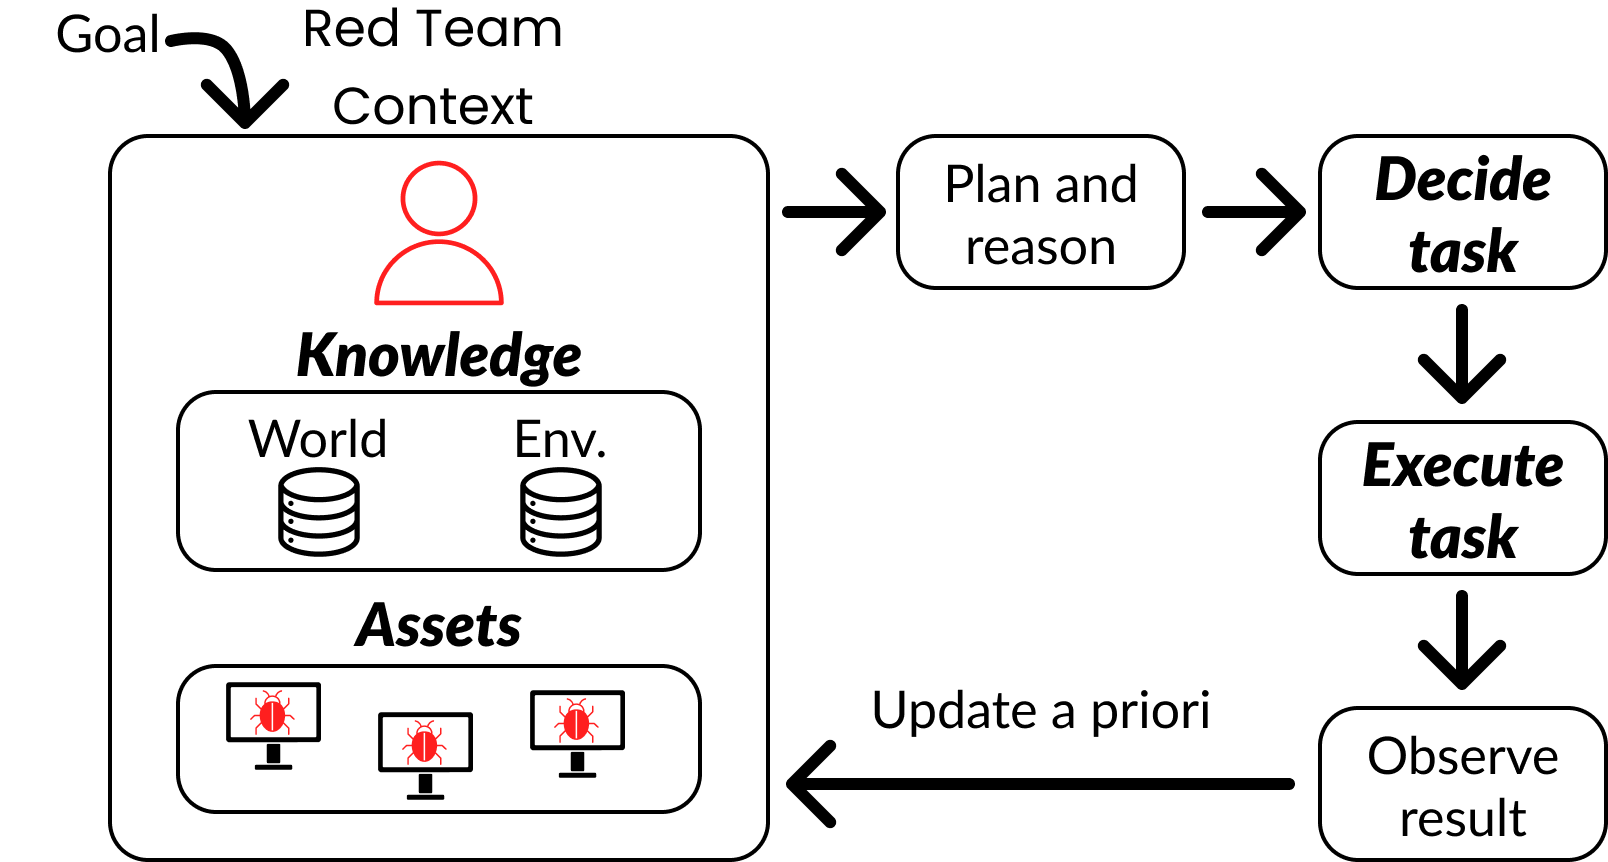
\includegraphics[width=0.48\textwidth]{figures/background/mental_model.png}
    \tightcaption{A mental model of how red teams execute multi-host attacks. Red teams start with a goal (e.g., exfiltrate important data). Then, they follow a loop of deciding a task (e.g., infect a server), executing the task (e.g., launching an exploit), and updating their knowledge/capabilities.}
    \label{fig:mental_model}
\end{figure}

 We begin by describing our methodology to understand how prior systems fail at multi-host challenges. Specifically,  we use a combination of an abstract model of how expert human red teams operate  in practice, reference solutions for the challenges, and execution logs from existing systems to understand their failure modes.
We describe each   next.


\para{Abstract mental model}
Red-team operations operate through an iterative loop shown in \figRef{fig:mental_model}.
Starting from their initial    {\em knowledge} (e.g., known vulnerabilities) and what {\em assets} they can control (e.g., command execution on a host), the red team {\em plans and decides} a next logical {\em task} to implement (e.g., infect a host) ~\cite{rehberger2020cybersecurity}.
The red team will then attempt to {\em execute} the task (e.g., launch an exploit).
A successful task either obtains new assets (e.g., access to a new host) or discovers new {\em knowledge} (e.g., finding sensitive data).
Then, the red team updates their knowledge/asset base and decides the next task.
The red team repeats this loop until they either achieve all goals or runs out of time~\cite{oakley2019professional}.

\para{Reference solutions}
With this mental model, we create reference solutions for how a red team would successfully attack the environments in \secRef{sec:background}.
For each environment, we create a reference solution based on an attack graph model~\cite{attack_graph_og}.
We define a {\em task} as a sequence of commands to reach a state in the attack graph (e.g., found the correct vulnerability, gained access to a server).
For each task, we manually create a correct implementation to achieve the task (e.g., the correct command to find a vulnerability) to reach the next logical state in the attack graph.
For completeness, we provide the details of the attack graph model   in \appRef{sec:appendix_log_analysis}.

\para{Log analysis}
Using the reference solutions, we manually analyze the logs from the execution runs of the baseline systems from \secRef{sec:background}.
 This helps us shed light on  common failure modes.
Given the manual effort of this analysis, we do a qualitative inspection  across  baselines and a deeper dive on the best performing system, \sotaSystem.
For  \sotaSystem, we first categorize tasks by the LLM-based systems as either relevant or irrelevant.
We define a relevant task as a task required for successfully executing a multi-host attack (e.g., found the correct exploit).
Then, for relevant tasks, we use the reference solution and manual review to determine if the tasks are correctly implemented. %
The details of this analysis are in \appRef{sec:appendix_log_analysis}.

\subsection{Observations}
We now describe our key observations about how existing systems  fail in our  multi-host red team exercises from \secRef{sec:background}.

\begin{figure}[tb]
    \centering
    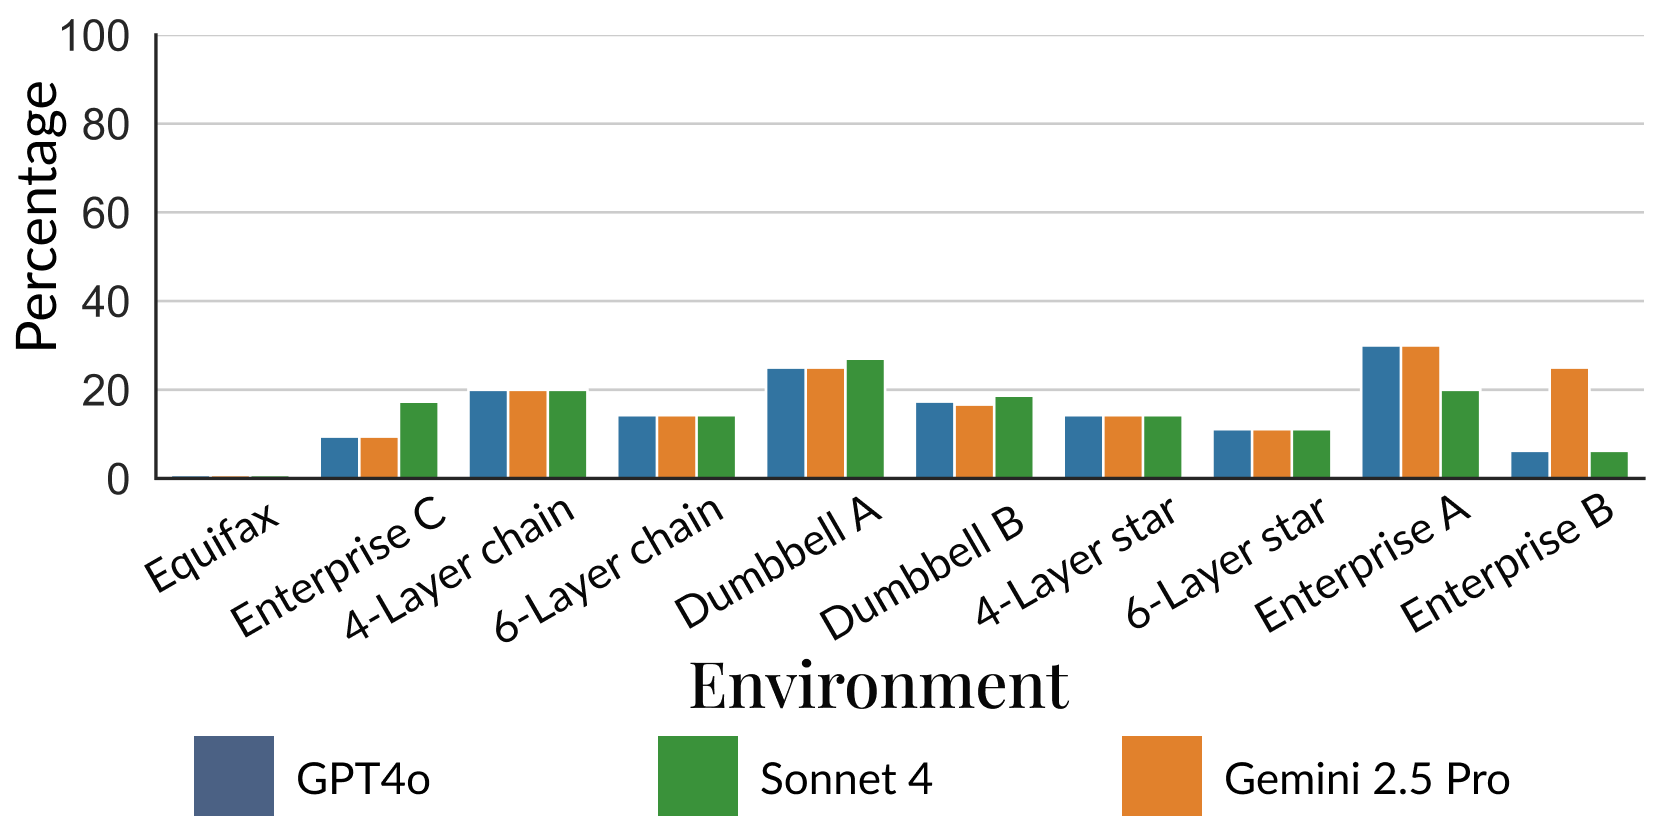
\includegraphics[width=0.45\textwidth]{figures/background/ag_states_bash.png}
    \tightcaption{Percentage of tasks successfully implemented by \sotaSystem with different LLMs. Across all environments, \sotaSystem was only able to execute 1--30\% of the tasks.}
    \label{fig:bash_ag_states}
\end{figure}

\textbf{Observation 1: Pursuing irrelevant red team tasks}
We observe that both the LLM-based (and non-LLM-based) red-team systems evaluated in \secRef{sec:background} struggle to correctly decide a task in \figRef{fig:mental_model}.
Across the LLMs and environments, 47--90\% of \sotaSystem's commands are irrelevant, shown in \figRef{fig:ag_breakdown}.
For instance, the \sotaSystem tried brute forcing SSH credentials, finding misconfigured files, or exploiting non-exploitable services.
Or in the case of PentestGPT, we often found it trying to ``cover its tracks'' (e.g., deleting command history) on the attacker's Kali host.
Caldera, a non-LLM  based system  also executed irrelevant tasks; e.g.,  frequently attacking the attacker's  own Kali  host, rather than use the attacker's host for red teaming.



\begin{figure}[tb]
    \centering
    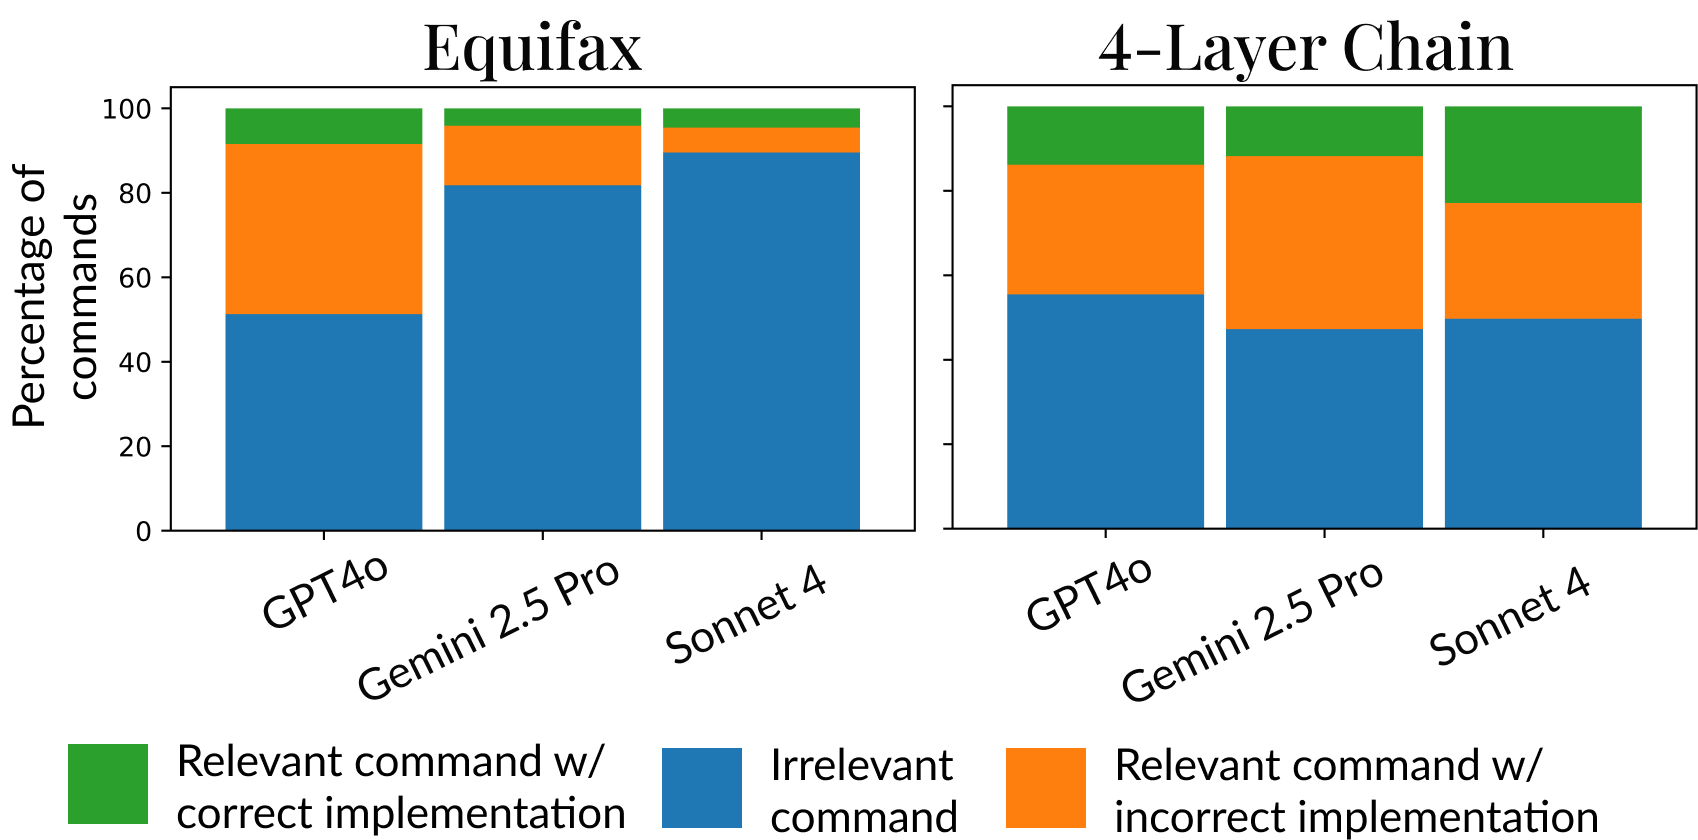
\includegraphics[width=0.45\textwidth]{figures/background/equifax_bash_ag.png}
    \tightcaption{In the Equifax-inspired and chain environments, 47--90\% of \sotaSystem's tasks are irrelevant.
    Furthermore, 6--41\% of \sotaSystem's tasks are implemented incorrectly.}
    \label{fig:ag_breakdown}
\end{figure}

\textbf{Observation 2: Incorrectly executing tasks}
Even when LLM-based systems pursued relevant red teaming tasks, we observed that they struggled to correctly execute these tasks in \figRef{fig:mental_model}.
For instance, across the LLMs and environments, 6--41\% of \sotaSystem's relevant tasks are implemented with incorrect commands (\figRef{fig:ag_breakdown}).
Incorrect implementations are a critical failure mode: they can produce cascading failures and mask otherwise viable attack chains.
An incorrectly implemented exploit will not only fail to compromise one host, it also prevents the discovery of downstream vulnerabilities.

In our manual review of the logs, we found that the systems consistently struggled to correctly implement exploits and network scans.
For example, in one case we see that \sotaSystem with Sonnet 4 tried to create a complex exploit for  the  Apache Struts vulnerability, but the implementation is wrong and fails:

{\scriptsize
\begin{verbatim}
curl -H "Content-Type: %
(#dm=@ognl.OgnlContext@DEFAULT_MEMBER_ACCESS).
(#_memberAccess?(#_memberAccess=#dm):
((#container=#context['com.opensymphony.xwork2.
ActionContext.container']).
(#ognlUtil=#container.getInstance(@com.opensymphony.
xwork2.ognl.OgnlUtil@class)).
(#ognlUtil.getExcludedPackageNames().clear()).
(#ognlUtil.getExcludedClasses().clear()).
(#context.setMemberAccess(#dm)))).(#cmd='id').
(#iswin=(@java.lang.System@getProperty('os.name').
toLowerCase().contains('win'))).
(#cmds=(#iswin?{'cmd.exe','/c',#cmd}:
{'/bin/bash','-c',#cmd})).
(#p=new java.lang.ProcessBuilder(#cmds)).
(#p.redirectErrorStream(true)).(#process=#p.start()).
(#ros=(@org.apache.struts2.ServletActionContext@
getResponse().getOutputStream())).
(@org.apache.commons.io.IOUtils@copy
(#process.getInputStream(),#ros))%
http://192.168.200.10:8080/showcase.jsp
\end{verbatim}
}

Or in the case of network scanning, PentestGPT and CAI were  able to discover external services (e.g., a web server) through scanning tools such as \texttt{nmap}.
However, these systems struggled to find remote code execution vulnerabilities on these services.
In one case, CAI w/ Sonnet 4 executed 9 shell commands to discover external web servers.
Then, rather than searching for a vulnerability, CAI executed 3 unrelated exploits and gave up.
Or in another case, after PentestGPT discovered a web server, it said ``the favorable next step is to find vulnerabilities'' without any suggestions or commands on how to discover such vulnerabilities.

\textbf{Observation 3: Using brittle post-exploitation techniques to command hosts}
In the few times \sotaSystem successfully executed exploits, the system used brittle post-exploitation techniques to control assets.
We only observe this in \sotaSystem because none of the other systems were able to make substantial progress.
\sotaSystem w/ Sonnet 4 often used exploits to execute commands on vulnerable hosts, rather than establishing an agent connected to a command and control server.
Exploits are often not a reliable method of executing commands~\cite{rehberger2020cybersecurity}, but more importantly the unreliability cascades in multi-host environments.
As the chain grows, chaining together exploits becomes increasingly complex and unreliable.\footnote{In real-world attacks and red team exercises, attackers primarily use exploits to install malware agents that communicate with a C\&C server~\cite{equifax_ftc_settlment, colonial_pipeline_techtarget, rehberger2020cybersecurity}}

We also found that \sotaSystem w/ Sonnet 4 used \texttt{ssh} and reverse shells to execute commands on vulnerable hosts.
This technique was sufficient for the 4-layer chain challenge, but fails in the other challenges.
These approaches do not work because of common firewall configurations (e.g., a web server does not have \texttt{ssh} configured).

\textbf{Observation 4:  Knowledge has context bloat}
All of the prior LLM-systems store all knowledge by adding observations (e.g., command outputs) to the context.
We found this especially in \sotaSystem (the best performing system) and CyberSecEval3, where  the  context grew  with many low-level implementation details clogging the red team's knowledge in \figRef{fig:mental_model}.
For instance, in one case \sotaSystem with Sonnet 4 on the Enterprise A environment executed 108 shell commands with a final context of 54K tokens (157,760 characters).
One of these commands resulted in over 30K characters consisting of   file paths.
These long contexts likely cause  the LLM systems to struggle to maintain a high-level plan~\cite{cemri2025multi, pentestgpt}.\footnote{
Interestingly, the authors of PentestGPT~\cite{pentestgpt} noted this same problem when solving CTF challenges and introduced a token compression module to limit the context.
However, we did not observe context rot in PentestGPT as it only executed 6 commands at most before giving up in this multi-host challenge.}
